
\section{Dimensionality Reduction}


The goal of this section is to introduce our first unsupervised learning task: \important{Dimensionality Reduction}. To do so we will introduce a linear dimensionality reduction technique, principal component analysis, and its kernel extension. We will also introduce autoencoders.


\begin{parag}{Until now: Supervised learning}
    Until this moment our model worked in two stages
	\begin{itemize}
		\item \textbf{Stage 1}: Training, we use the data with ground truth labels to optimize model parameters
		\item \textbf{Stage 2}: Testing, we predict the output for a new data sample (with the fixed parameters)
	\end{itemize}
	Supervised learning is good when we have a concrete prediction task to solve and labelled data. However it is not suited when we don't have labels and when we are trying to get an understanding of the data.
\end{parag}

\begin{parag}{Unsupervised learning}
    Today, we will do it differently, we will have only a single state which transforms the data for further analysis.

	\begin{center}
	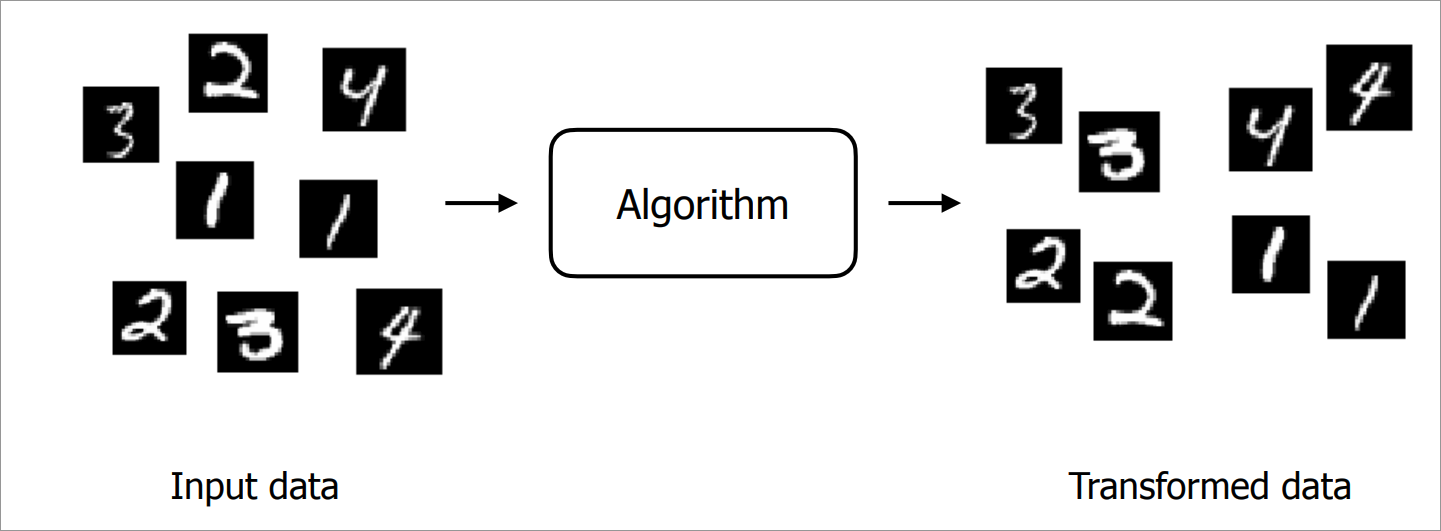
\includegraphics[scale=0.2]{screenshots/2026-05-05_1.png}
	\end{center}
\end{parag}


\begin{parag}{Dimensionality Reduction}
    To have a better understanding let us introduce it via an example, \important{data size reduction}. Let us have a vectorized image, a huge vector:
	\begin{align*} 
		x_i \in \mathbb{R}^{536 \cdot 356 \cdot  3} = \mathbb{R}^{572448}
	\end{align*}
	Dealing with such large data is cumbersome, is there a way for us to compress it while keeping the relevant information?\\
	$ $\\
	Another example would be by images created by translating an rotating the same digit $3$
	\begin{center}
	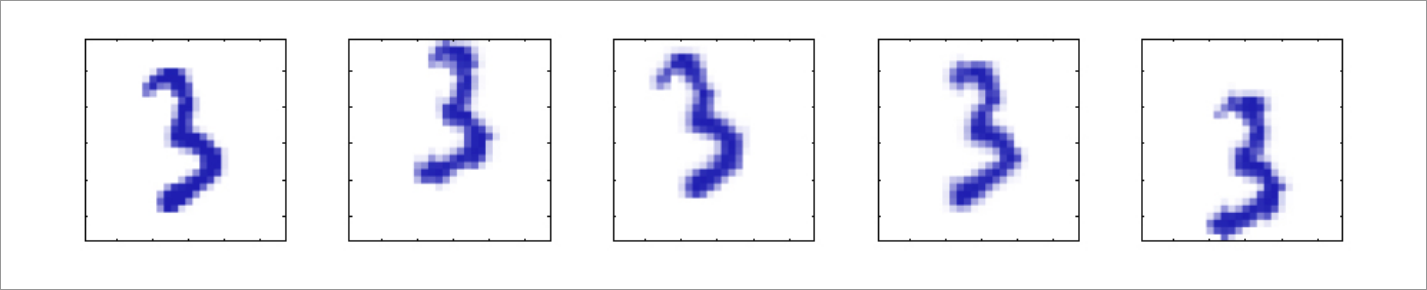
\includegraphics[scale=0.2]{screenshots/2026-05-05_2.png}
	\end{center}
	This data lies in a high dimensional space ($32 \times 32$). However there is only $3$ degrees of freedom here (2 translations and 1 rotation). Inherently this data lies in a $3$ dimensional space. In practice, the data often lies in a much lower dimensional space, referred to as manifold.
	\begin{definition}{Dimensionality Reduction}
	Dimensionality reduction is the task of 
	\begin{itemize}
	    \item Discovering the data manifold
	    \item Getting a low-dimensional representation of the data
			\begin{itemize}
			\item Sometimes at some loss of information (hopefully loss)
			\end{itemize}
	\end{itemize}
	\end{definition}
	\begin{center}
	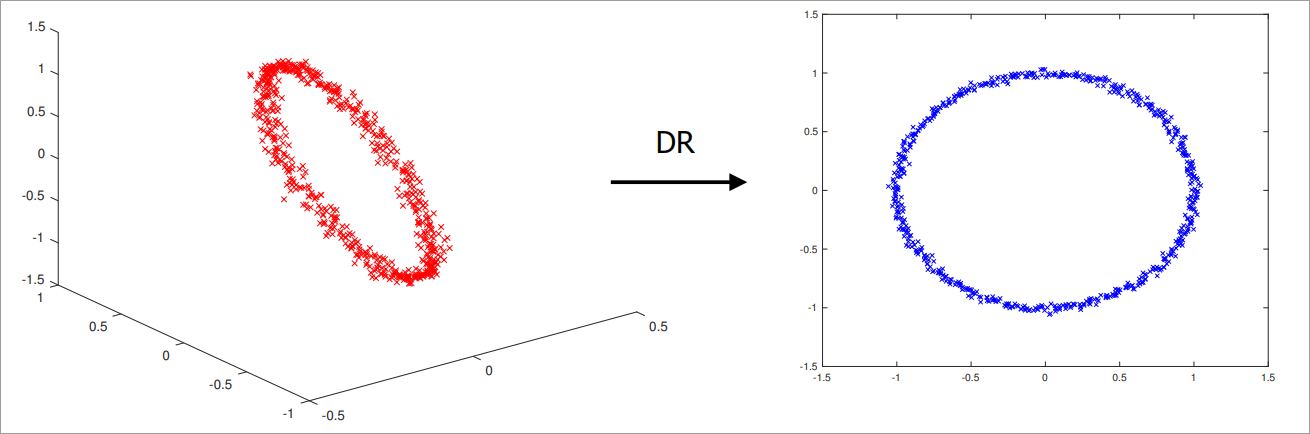
\includegraphics[scale=0.2]{screenshots/2026-05-05_3.png}
	\end{center}
	Therefore we have as input $x_i \in \mathbb{R}^{D}$ and as output $y_i \in \mathbb{R}^{d}$ where $D \gg d$. Our goal is to find a mapping 
	\begin{align*} 
		y_i = f\left(x_i\right)
	\end{align*}
	Let us try first with a linear one:
	\begin{align*} 
		y_i = W^{T}x_i
	\end{align*}
\end{parag}

\begin{parag}{Principal Component Analysis (PCA)}
    Given $N$ samples $\left\{x_i\right\}$, PCA yields a projection of the form 
	\begin{align*} 
		y_i =  W^{T}\left(x_i - \overline{x}\right) \mathspace \mathspace \text{ s.t. } W^{T}W =  I_d
	\end{align*}
	where $\overline{x}$ is the mean of the data 
	\begin{align*} 
		\overline{x} = \frac{1}{N} \sum_{i= 1}^{N}x_i
	\end{align*}
	Okay sure why not, but the data is \important{unsupervised} so we don't have and other test label $y_i$ that we can refer to in order to train our model. The question that this brings is: \textit{What do we want this projection to achieve}?
\end{parag}

\begin{parag}{PCA: Objective}
	We want two things 
	\begin{itemize}
	    \item Keep most of the '\textit{important}' signal
	    \item Remove the noise
	\end{itemize}
	This can be achieved by finding directions that have a large variance, i.e., for the $j^{\text{th}}$ output dimension, we want to maximize 
	\begin{align*} 
		\text{var}\left(\left\{y_i^{\left(j\right)}\right\}\right) = \frac{1}{N} \sum_{i= 1}^{N}\left(y_i^{\left(j\right)} - \overline{y}^{\left(j\right)}\right)^2
	\end{align*}
	Where $\overline{y}^{\left(j\right)}$ is the mean of the $j^{\text{th}}$ dimension of the data after projection.
\end{parag}


\begin{parag}{Variance maximization}
    Let us look at the projection to a 1D space. That is, we use a vector $D$-dimensional $w_{\left(1\right)}$ such that $w_{\left(1\right)}^{T}w_{\left(1\right)} = 1$ instead of a matrix $W \in \mathbb{R}^{D \times d}$\\
	$ $\\
	In this case, the mean of the data after projection is 
	\begin{align*} 
		\overline{y} &=  \frac{1}{N} \sum_{i= 1}^{N} y_i = \frac{1}{N} \sum_{i= 1}^{N}w_{\left(1\right)}^{T}\left(x_i - \overline{x}\right)\\
		&= w_{\left(1\right)}^{T} \left(\frac{1}{N}\sum_{i= 1}^{N}x_i\right) - w_{\left(1\right)}^{T}\overline{x} = 0
	\end{align*}
	Then for the variance of the data projection, 
	\begin{align*} 
		\text{var} \left(\left\{y_i\right\}\right) &= \frac{1}{N} \sum_{i= 1}^{N} \left(y_i - \overline{y}\right)^2 = \frac{1}{N} \sum_{i= 1}^{N} \left(w_{\left(1\right)}^{T}\left(x_i - \overline{x}\right) - 0\right)^2 \\
												   &= \frac{1}{N} \sum_{i= 1}^{N} \left(w_{\left(1\right)}^{T}\left(x_i \overline{x}\right)\right)^2 =  \frac{1}{N} \sum_{i= 1}^{N} w_{\left(1\right)}^{T}\left(x_i - \overline{x}\right)\left(x_i - \overline{x}\right)^{T}w_{\left(1\right)}\\
												   &= w_{\left(1\right)}^{T}\left(\frac{1}{N}\sum_{i= 1}^{N}\left(x_i - \overline{x}\right)\left(x_i - \overline{x}\right)^{T}\right)w_{\left(1\right)} =  w_{\left(1\right)}^{T}Cw_{\left(1\right)}
	\end{align*}
	Where $C$ is the input data covariance matrix 
	\begin{align*} 
		C = \frac{1}{N} \sum_{i= 1}^{N}\left(x_i - \overline{x}\right) \left(x_i - \overline{x}\right)^{T}
	\end{align*}
	Therefore what we seek to solve is the problem 
	\begin{align*} 
		\max_{w_{\left(1\right)}} w_{\left(1\right)}^{T}Cw_{\left(1\right)}\\
		\text{ s.t. } w_{\left(1\right)}^{T}w_{\left(1\right)} = 1
	\end{align*}
	To do so, we can write the Langrangian of this problem (don't ask why)
	\begin{align*} 
		\mathcal{L}\left(w_{\left(1\right)}, \lambda_i\right) = w_{\left(1\right)}^{T} Cw_{\left(1\right)} + \lambda_1 \left(1 - w_{\left(1\right)}^{T}w_{\left(1\right)}\right)
	\end{align*}
	Setting the gradient of the Lagrangian w.r.t. $w_{\left(1\right)}$ to $0$ yields 
	\begin{align*} 
		Cw_{\left(1\right)} =  \lambda_1 w_{\left(1\right)}
	\end{align*}
	This is the definition of an eigenvector. Therefore $w_{\left(1\right)}$ must be an eigenvector of $C$, with eigen value $\lambda_1$
	\begin{framedremark}
		Let us just do the calculation:
		\begin{align*} 
			\nabla_{w} \mathcal{L} = 2Cw - 2\lambda w =  0 \implies Cw =  \lambda w
		\end{align*}
	\end{framedremark}
	However which eigenvector? By multiplying both sides of the eigenvector equation from the left by $w_{\left(1\right)}^{T}$ yields 
	\begin{align*} 
		w_{\left(1\right)}^{T}Cw_{\left(1\right)} =  \lambda \underbrace{w_{\left(1\right)}^{T}w_{\left(1\right)}}_{= 1} = \lambda_1
	\end{align*}
	The resulting term of the left hand side is the variance of the projected data. Since we seek to maximize it, we should take $w_{\left(1\right)}$ as the eigen vector corresponding to the largest eigenvalue $\lambda_1$
\end{parag}

\begin{parag}{Dealing with more that 1D projections}
    To obtain an output representation that is more than 1D, i.e., $d > 1$, we can perform recursively 
	\begin{itemize}
	    \item The second projection vector $w_{\left(2\right)}$ corresponds to the eigenvector of $C$ with the second largest eigenvalue
	    \item The third vector $w_{\left(3\right)}$ with the eigenvector with the third largest eigenvalue
	    \item $\ldots$
	\end{itemize}
	The matrix $W$ is obtained by concatenating the resulting vectors 
	\begin{align*} 
		W =  \left[w_{\left(1\right)} \mathspace w_{\left(2\right)} \mathspace \cdots \mathspace w_{\left(d\right)}\right] \in \mathbb{R}^{D \times d}
	\end{align*}
	this guarantees to satisfy the constraint $W^{T}W =  I_d$ (as eigenvectors of a matrix are orthogonal and of norm $1$)\\
	$ $\\
	In the limit, one can use all dimensions, i.e., set $d = D$, this implies
	\begin{itemize}
	    \item There is therefore no reduction of dimensionality
	    \item In 3D, we can think of this as a rotation of the data
	    \item This incurs no loss of information
	    \item The $d =  D$ dimensions in the new space are uncorrelated
	\end{itemize}
	Another option is to keep all the eigenvectors that correspond to non-zero eigenvalues.
	\begin{itemize}
	    \item This means that the data is truly low-dimensional
	    \item E.g., this happens when we have fewer samples than dimensions ($N < D$)
	    \item The resulting $\left\{y_i\right\}$ are lower dimensional $\left(d < D\right)$
	    \item But there is no loss of information.
	\end{itemize}
	
	
\end{parag}

In practice, one typically truncates the eigenvalues so as to discard some that are non-zero 
\begin{itemize}
    \item This can be achieved by aiming to retain a pre-defined percentage of the data variance, measured as the sum of eigenvalues
    \item E.g. to retain at least $90\%$ of the variance, one can search for $d$ such that 
		\begin{align*} 
			\sum_{j = 1}^{d}\lambda_j \geq 0.9 \sum_{k= 1}^{D} \lambda_k
		\end{align*}
		Assuming the eigenvalues are sorted in decreasing order. The resulting $\left\{y_i\right\}$ have an even lower dimension.
\end{itemize}


\begin{parag}{Error minimization}
    This incurs some loss of information
	\begin{center}
	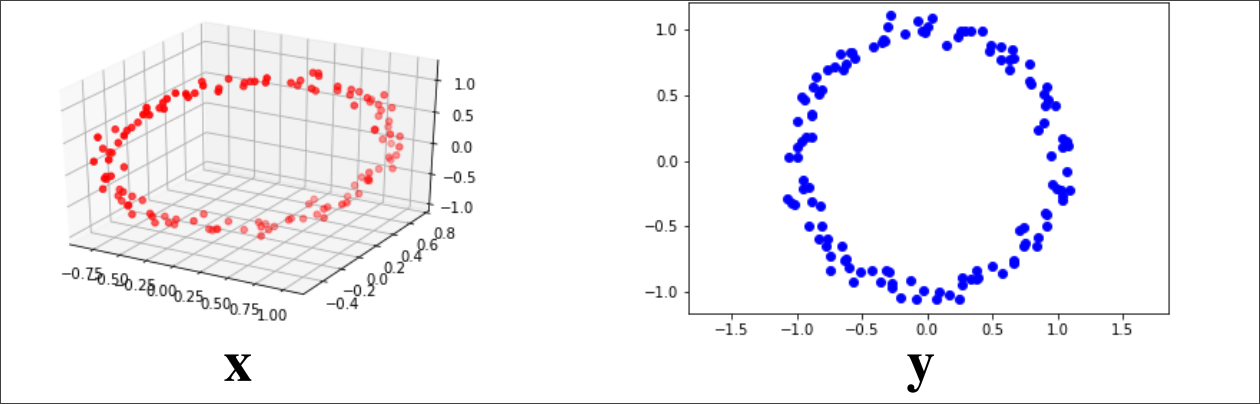
\includegraphics[scale=0.2]{screenshots/2026-05-05_4.png}
	\end{center}
	However the corresponding matrix $W$ is the orthogonal matrix that minimizes the reconstruction error 
	\begin{align*} 
		e_i =  \left\|\hat{x}_i - x_i\right\|^2
	\end{align*}
	where 
	\begin{align*} 
		\hat{x}_i =  \overline{x} + Wy_i =  \overline{x} WW^{T}(x_i - \overline{x})
	\end{align*}

\end{parag}






\begin{parag}{Mapping}
    PCA not only reduces the dimensionality of the original data. It provides a continuous mapping from the low-dimensional space to the high-dimensional one. That is, for any $y \in \mathbb{R}^{d}$, we can compute a point in the high-dimensional space as 
	\begin{align*} 
		\hat{x} =  \overline{x} + Wy
	\end{align*}
	This mapping constrains $\hat{x}$ to lie in a subspace, and thus provides a form of regularization. 
\end{parag}

\begin{parag}{Dealing with nonlinear data}
    Here all we have done is still linear, PCA is a linear dimensionality reduction method (it just gives projections of the data). How can we achieve nonlinear dimensionality reduction 
	\begin{center}
	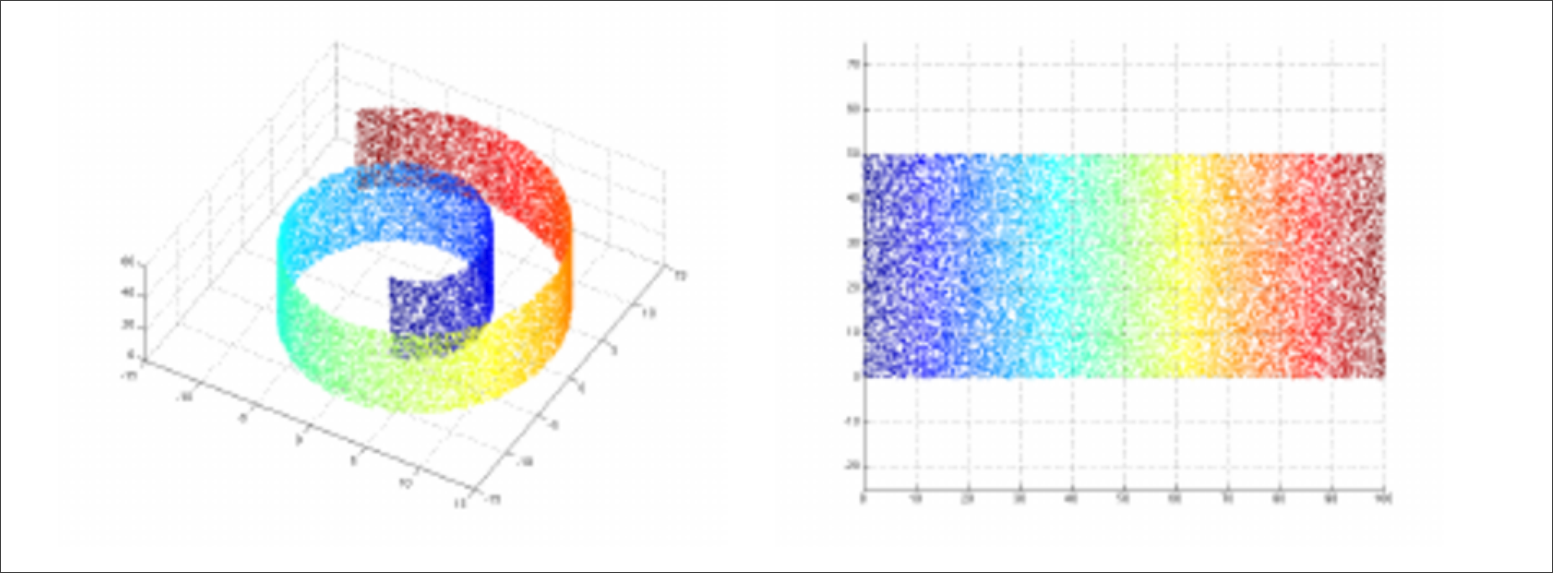
\includegraphics[scale=0.2]{screenshots/2026-05-05_5.png}
	\end{center}
\end{parag}


\begin{parag}{Kernel PCA}
    We will use the same intuition as in Supervised kernel methods, we will use a map to high dimensional space
	\begin{align*} 
		x_i \to \phi(x_i)
	\end{align*}
	And then perform PCA on it.\\
	$ $\\
	Our goal will again be to replace dot products with kernel values 
	\begin{align*} 
		k\left(x_i, x_j\right) = \phi\left(x_i\right)^{T}\phi\left(x_j\right)
	\end{align*}
	Let us first assume that the data is centred in feature space. That is 
	\begin{align*} 
		\frac{1}{N} \sum_{i= 1}^{N}\phi\left(x_i\right) = 0
	\end{align*}
	Then, the covariance matrix can be written as 
	\begin{align*} 
		C = \frac{1}{N} \sum_{i= 1}^{N}\phi\left(x_i\right)\phi\left(x_i\right)^{T}
	\end{align*}
	Note that this is an $F \times F$ matrix, not an $N \times N$ one, so we still do not have kernel values here.\\
	$ $\\
	Applying PCA in feature space means that we need to solve the eigenvalue problem 
	\begin{align*} 
		Cw_{\left(1\right)} = \lambda_1 w_{\left(1\right)}
	\end{align*}
	Where $w_{\left(1\right)}$ now is an $F$-dimensional vector. From the previous definition of $C$, this can be written as 
	\begin{align*} 
		\left(\frac{1}{N}\sum_{i= 1}^{N}\phi\left(x_i\right)\phi\left(x_i\right)^{T}\right)w_{\left(1\right)} = \lambda_1 w_{1}
	\end{align*}
	Recall from the Representer theorem, $w_{\left(1\right)}$ can be expressed as a linear combination of the $\left\{\phi\left(x_i\right)\right\}$ i.e.,  
	\begin{align*} 
		w_{\left(1\right)} = \sum_{j = 1}^{N}a_j \phi\left(x_j\right)
	\end{align*}
	Let us then substitute this alternative representation of $w_{\left(1\right)}$ in our eigenvector equation. This yields 
	\begin{align*} 
		\left(\frac{1}{N}\sum_{i= 1}^{N}\phi\left(x_i\right)\phi\left(x_i\right)^{T}\right)\sum_{j= 1}^{N}a_j \phi\left(x_j\right) = \lambda_1 \sum_{j= 1}^{N}a_j \phi\left(x_j\right)
	\end{align*}
	After some computations (skipped here), we can obtain a new eigenvalue problem 
	\begin{align*} 
		Ka =  \lambda_1 Na
	\end{align*}
	Where $a \in \mathbb{R}^{N}$ is the vector containing the new parameters of the problem, and $K$ is the kernel matrix.\\
	$ $\\
	Solving this problem gives us a vector $a$, from which we could, in theory, obtain $w_{\left(1\right)}$ as 
	\begin{align*} 
		w_{\left(1\right)} =  \sum_{i= 1}^{N}a_i \phi\left(x_i\right)
	\end{align*}
	Note, However, that it depends on $\left\{\phi\left(x_i\right)\right\}$ which are unknown.\\
	$ $\\
	As in kernel ridge regression, this can be addressed by noting that, ultimately, we are not interested in $w_{\left(1\right)}$, but rather in obtaining the low-dimensional projections $\left\{y_i\right\}$.\\
	$ $\\
	For 1D representation, these projections can be computed as 
	\begin{align*} 
		y_i =  \phi\left(x_i\right)^{T}w_{\left(1\right)} =  \sum_{ j = 1}^{N} a_j \phi\left(x_i\right)\phi\left(x_i\right)^{T} = \sum_{j =  1}^{N}a_j k\left(x_i, x_j\right)
	\end{align*}
	Which depends on the kernel function $k$. As in the linear case, multiple output dimensions can be obtained by taking the $d$ eigenvectors with largest eigenvalues
\end{parag}


\begin{parag}{Non centred data}
    So far, we have assumed that the data was centred in feature space. There is however no reason for this to be satisfied 
	\begin{itemize}
	    \item Even is the original data is centred, the data after the mapping to feature space might not be
	\end{itemize}
	To handle more realistic scenario, where it isn't, let us define 
	\begin{align*} 
		\widetilde{\phi}\left(x_i\right) = \phi\left(x_i\right) - \frac{1}{N} \sum_{j = 1}^{N}\phi\left(x_j\right)
	\end{align*}
	The $\left(i, j\right)^{\text{th}}$ elements of the corresponding kernel matrix is then given by 
	\begin{align*} 
		\widetilde{K}_{i, j} = \left(\widetilde{\phi}\left(x_I\right)\right)^{T}\widetilde{\phi}\left(x_j\right)
	\end{align*}
	This kernel matrix can in fact be computed based on the original one as 
	\begin{align*} 
		\widetilde{K} =  K - 1_N K - K1_N + 1_NK1_N
	\end{align*}
	Where $1_N$ is an $N \times N$ matrix with every element equal to $\frac{1}{N}$
	

\end{parag}


\begin{parag}{Example}
    Here are a couple of examples on how that look like:
	Swiss roll: PCA results
	\begin{center}
	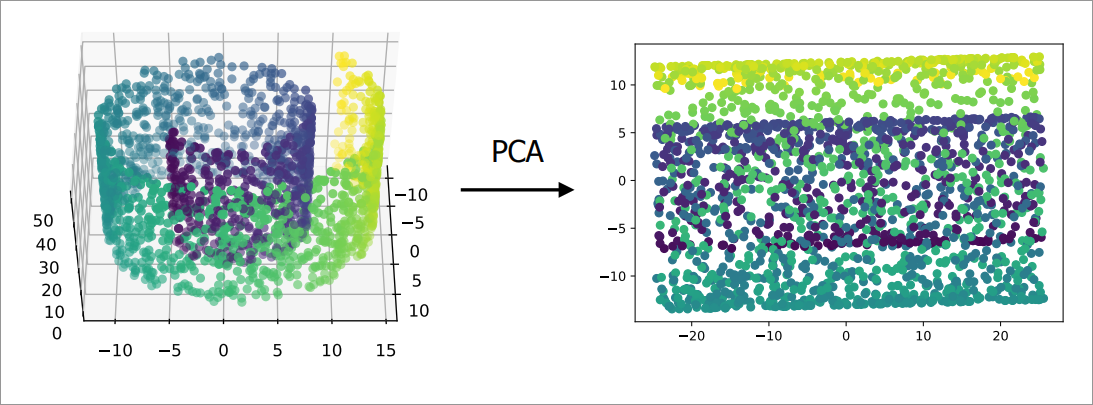
\includegraphics[scale=0.3]{screenshots/2026-05-05_6.png}
	\end{center}
	Using a RBF kernel now 
	\begin{center}
	\includegraphics[scale=0.3]{screenshots/2026-05-05_7png}
	\end{center}
	3D inputs, 2 classes: PCA resulting 
	\begin{center}
	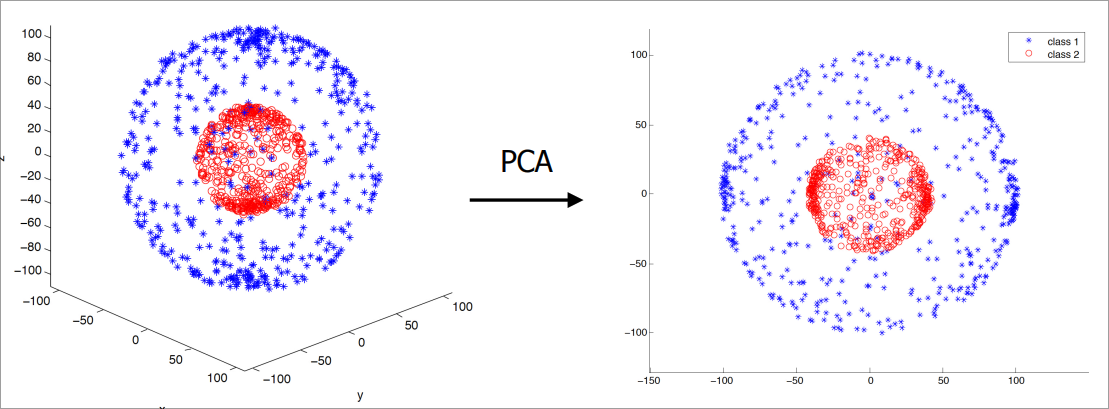
\includegraphics[scale=0.3]{screenshots/2026-05-05_8.png}
	\end{center}
	Using the same data but with a RBF kernel 
	\begin{center}
	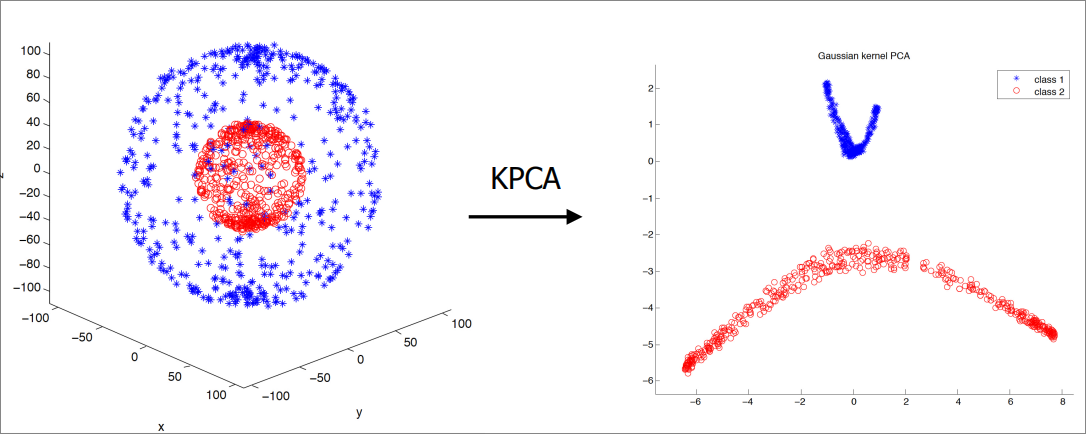
\includegraphics[scale=0.3]{screenshots/2026-05-05_9.png}
	\end{center}
	Here we can see that RBF kernel are pretty good here, but why?
\end{parag}


\begin{parag}{Kernel PCA vs PCA}
    As PCA, Kernel PCA defines a mapping from the high-dimensional data to the low dimensional one. However, in contrast to PCA, Kernel PCA does not provides a mapping from the low-dimensional space to the high-dimensional one. 
	\begin{itemize}
	    \item We cannot simply compute the high-dimensional version of any point in the low dimensional space
	\end{itemize}
	Can we nonetheless have this inverse mapping with nonlinear methods? The solution is to rely on deep networks
	\begin{subparag}{Another look at PCA}
	    PCA provides a mapping from high to low dimension and back
		\begin{align*} 
			x \to y = W^{T}\left(x - \overline{x}\right) \to \hat{x} = \overline{x} + Wy
		\end{align*}
		Both mappings are linear, so PCA cannot handle nonlinear $\to$ linear $\to $ non linear
	\end{subparag}
	In order to use deep networks, we will introduce \important{autoencoder}
\end{parag}

\subsection{Autoencoder}
We have used linear mapping before but there is no reason to limit ourselves to linear, therefore following neural networks, the simplest extension consists of using a nonlinear activation function in the middle. This is referred to as an \important{autoencoder}.

\begin{center}
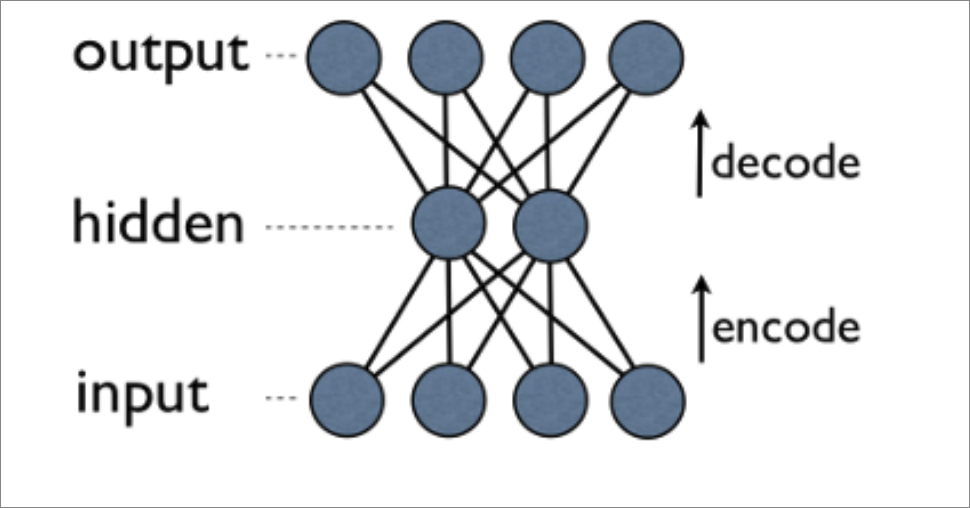
\includegraphics[scale=0.2]{screenshots/2026-05-05_10.png}
\end{center}
\begin{align*} 
	\hat{x} =  Wf\left(W^{T}x\right)
\end{align*}
with $f$ being a nonlinear, element wise activation function.



\begin{parag}{General form}
    In general, an autoencoder can be represented by two mappings
	\begin{itemize}
	    \item The encoder going from the input to a latent representation
	    \item The decoder going from the latent representation to the output
	\end{itemize}
	\begin{center}
	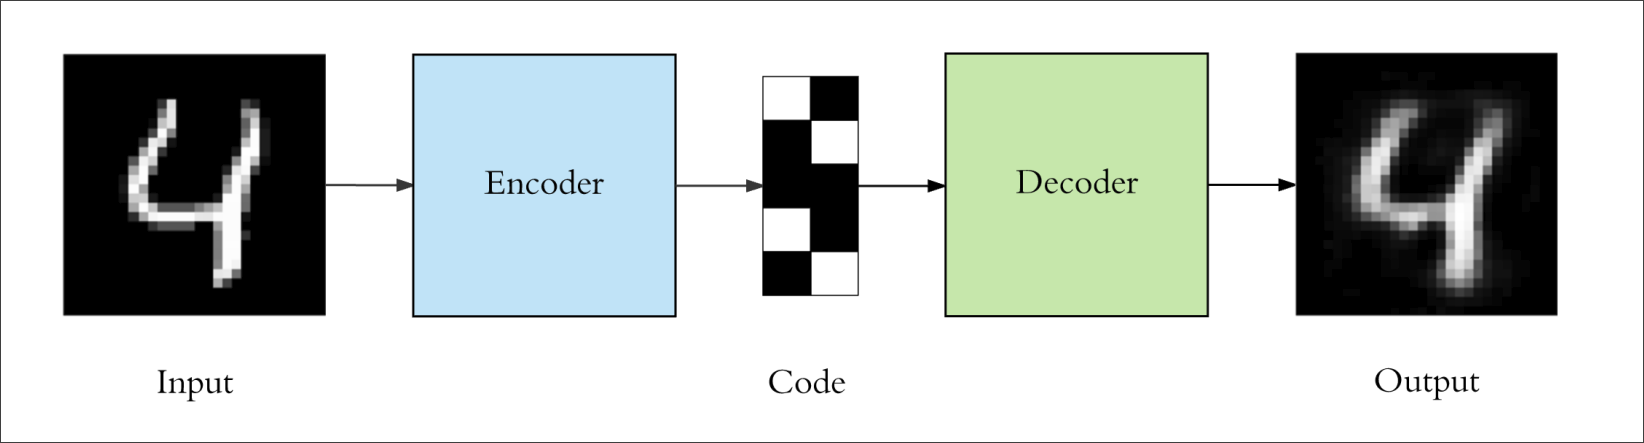
\includegraphics[scale=0.2]{screenshots/2026-05-05_11.png}
	\end{center}
	As in the PCA case, the output of the decoder is meant to be similar to the original input
\end{parag}


\begin{parag}{Deep autoencoder}
    And as previous, there is no reason to restrict the encoder and decoder to consist of a single layer, we can then create deep autoencoders by stacking multiple layers each with an activation function.\\
	$ $\\
	Each layer gives a mapping of the form
	\begin{align*} 
		z_{\left(j\right)} =  f_{\left(j\right)}\left(W_{\left(j\right)}^{T}z_{\left(j-1\right)}\right)
	\end{align*}
	\begin{center}
	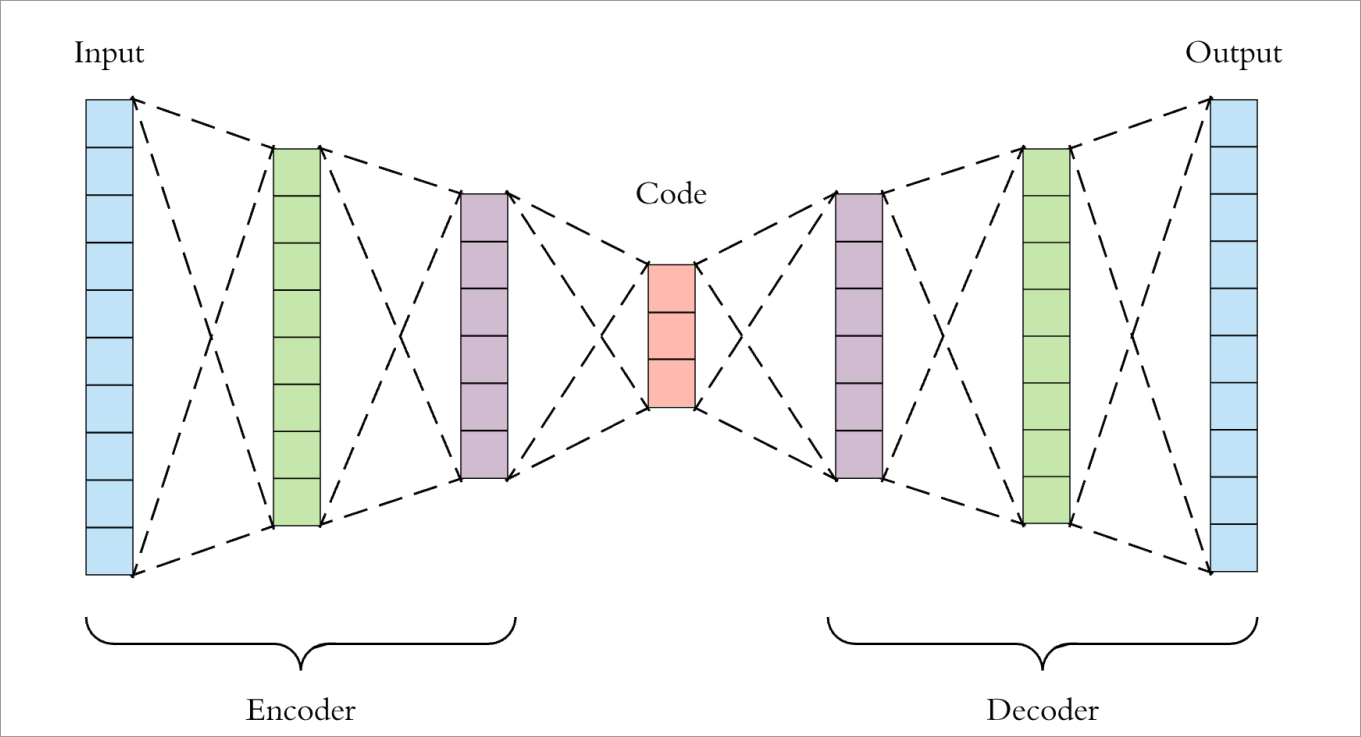
\includegraphics[scale=0.2]{screenshots/2026-05-05_12.png}
	\end{center}
\end{parag}

\begin{parag}{Training}
    As mentioned before, with PCA, the reconstructed inputs $\left\{\hat{x}_i\right\}$ minimize the least square error 
	\begin{align*} 
		e_i =  \left\|\hat{x}_i - x_i\right\|^2
	\end{align*}
	following this intuition, an autoencoder can be trained by minimizing the empirical risk 
	\begin{align*} 
		R\left(\left\{W_{\left(j\right)}\right\}\right) = \frac{1}{N} \sum_{i= 1}^{N} \left\|\hat{x}_i \left(\left\{W_{\left(j\right)}\right\}\right) - x_i\right\|^2
	\end{align*}
	As for MLPs, this is non convex and the minimization process is done via stochastic gradient descent.
\end{parag}


\begin{parag}{Dimensionality expansion}
    Because the mapping is nonlinear, there is no reason to restrict (again...) the laten representation to be low dimensional. One can then perform dimensionality expansion 
	\begin{center}
	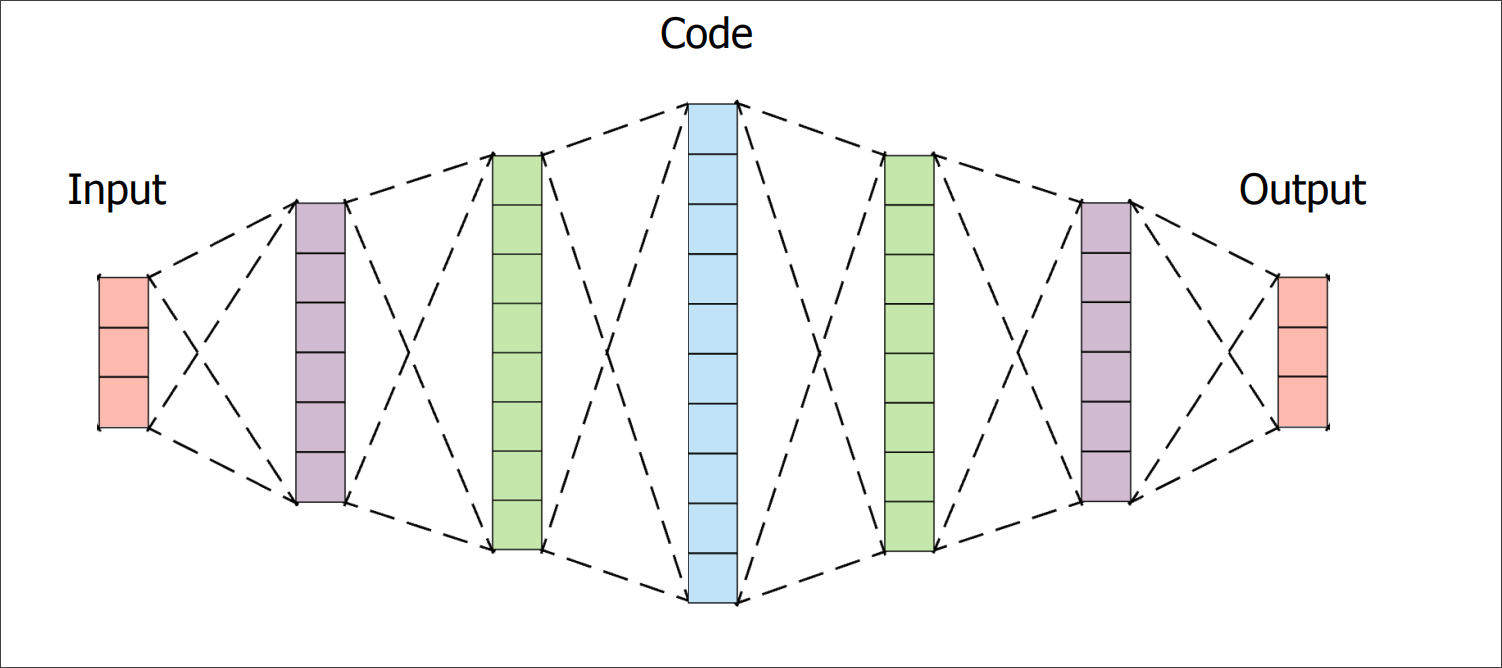
\includegraphics[scale=0.2]{screenshots/2026-05-05_13.png}
	\end{center}

\end{parag}


\begin{parag}{Denoising autoencoders}
    Having a low-dimensional laten representation encourages the autoencoder to learn an '\textit{intelligent}' mapping. With dimensionality expansion, one could simply learn to copy the input. To avoid this, one can add noise to the input and aim to reconstruct a noise-free version of the input.
	\begin{center}
	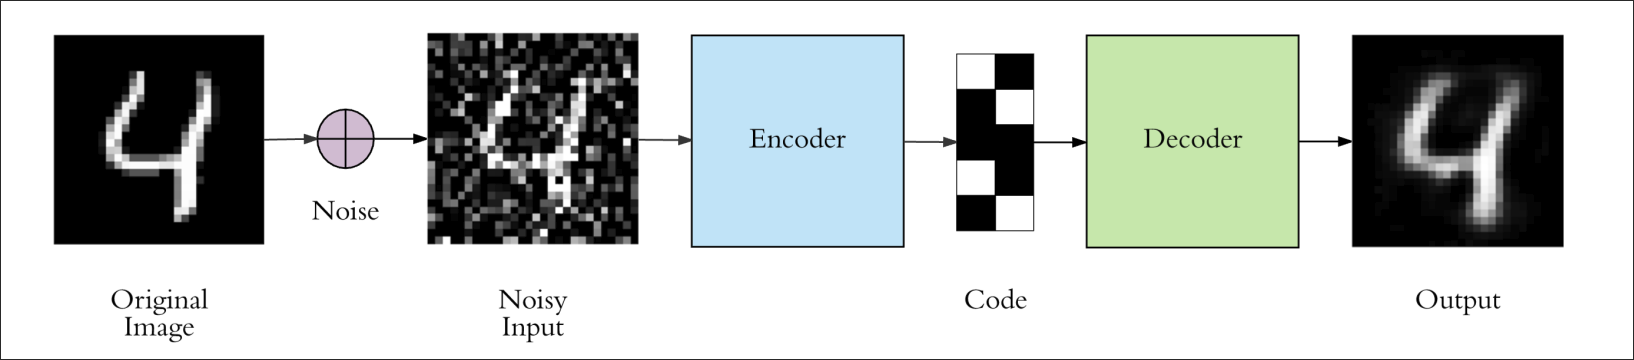
\includegraphics[scale=0.2]{screenshots/2026-05-05_14.png}
	\end{center}
\end{parag}

\begin{parag}{Sparse autoencoder}
    Another approach to learn a meaningful latent representation consists of adding a regularizer. 
	\begin{itemize}
	    \item Let $y_i$ denote the latent representation (or code) for sample $i$
	    \item Then, one can encourage a large number of the elements $\left\{y_i^{\left(k\right)}\right\}$ to go to zero
	    \item This can be achieved by a sparsity-including regularizer, such as the $L_1$ norm 
			\begin{align*} 
				E_{r}\left(\left\{W_{\left(j\right)}\right\}\right) =  \sum_{i= 1}^{N}\sum_{k= 1}^{M}\left|y_i^{\left(k\right)}\right|
			\end{align*}
	\end{itemize}
	With $M$ dimensionality of the latent representation
\end{parag}


\begin{parag}{Convolutional autoencoder}
	With convolutions and upsampling-convolutions, or transposed convolutions, one can also design convolutional autoencoders. Note that fully connected layers can also be used in the middle 
	\begin{center}
	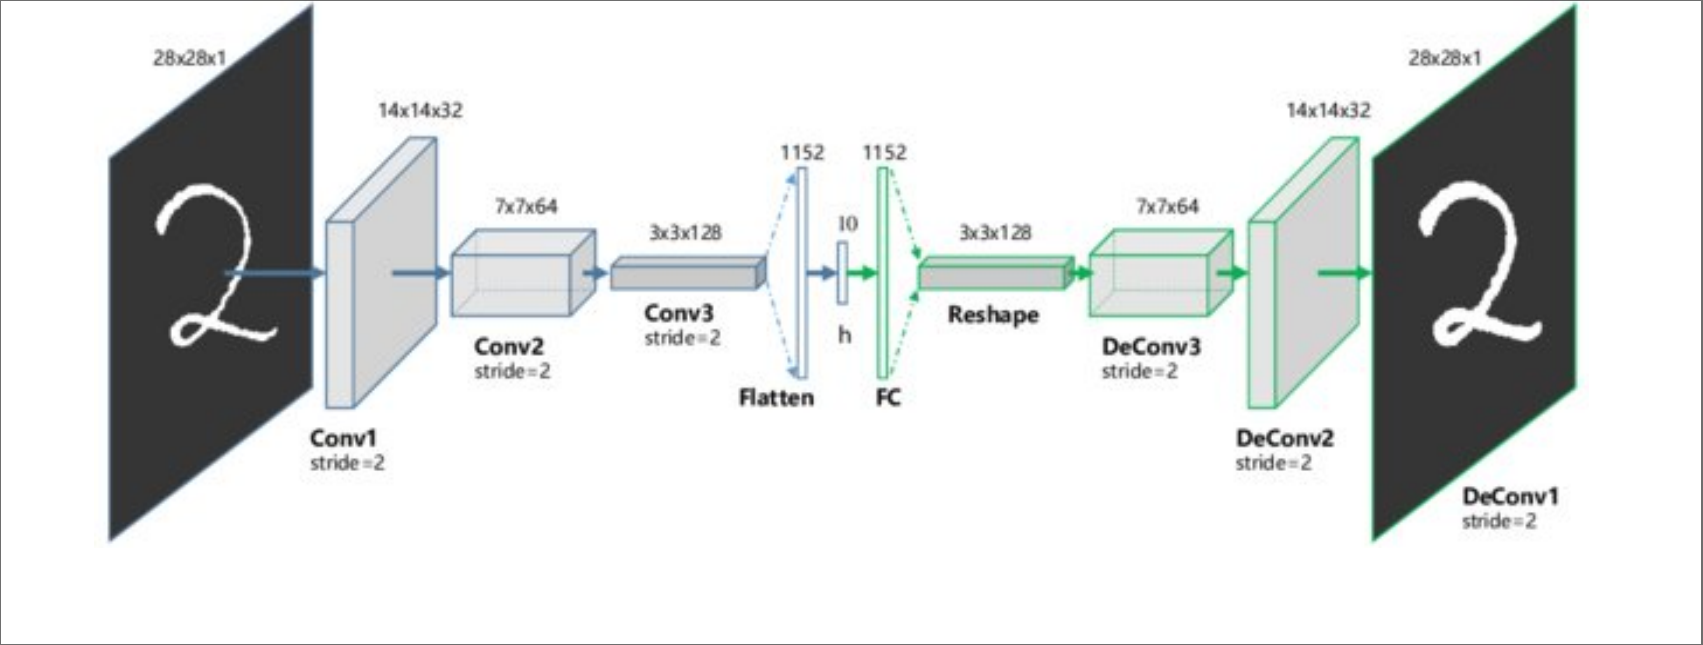
\includegraphics[scale=0.15]{screenshots/2026-05-05_15.png}
	\end{center}
\end{parag}


\begin{parag}{Autoencoder: Application}
    A code provides a compact representation of the input. It can be used for retrieval in a large data collection, e.g., via $k$ nearest neighbours.
\end{parag}



\begin{parag}{Mapping}
    As in PCA, the decoder provides a mapping from the latent space to the output (same as input) space. One can thus generate new samples (e.g., images) by taking arbitrary points in the latent space
	\begin{center}
	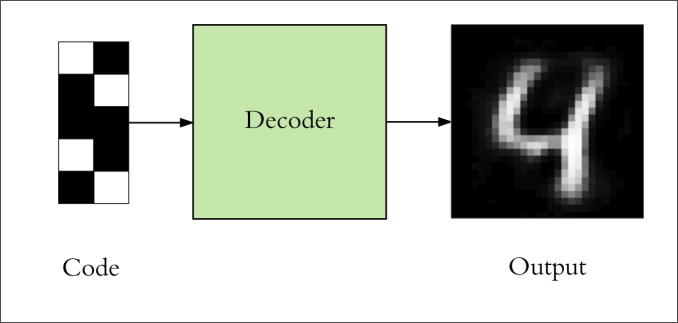
\includegraphics[scale=0.3]{screenshots/2026-05-05_16.png}
	\end{center}
\end{parag}


















